\subsection{Phase Independent intervals Algorithms}
\label{SubsectionShapelet}
Phase independent intervals, or just shapelets as less formally known,
are subseries which are ultimately distinctive of classes regardless of their place on the time series \cite{schafer2017fast,bagnall2017great}.
They were first introduced in \cite{ye2009time} as an alternative for KNN approaches; to overcome their shortcomings.

Shapelets reduce the space and time complexity needed by KNN, because they are formed from subsequences which are shorter than
the original time series. Needing only one shapelet at classification time, they form a compressed format of the classification problem \cite{bostrom2017shapelet,ye2009time,mueen2011logical}.
While KNN classify based on comparison to other instances, shapelets provide insight about the unique features of classes and thus more
interpretable results of how the classification was carried out.
Finally, shapelets are best suited for problems where a certain pattern can differentiate instances which is harder to detect when comparing whole series \cite{bagnall2017great,Bostrom2017}.
Figure \ref{Img:Shapelet} shows how shapelets can separate instances by calculating distances and provide interpretable explanation by projecting the data in a shapelet transform space.

\begin{figure}[!htbp]
    \captionsetup{justification=raggedright}
    \centering
    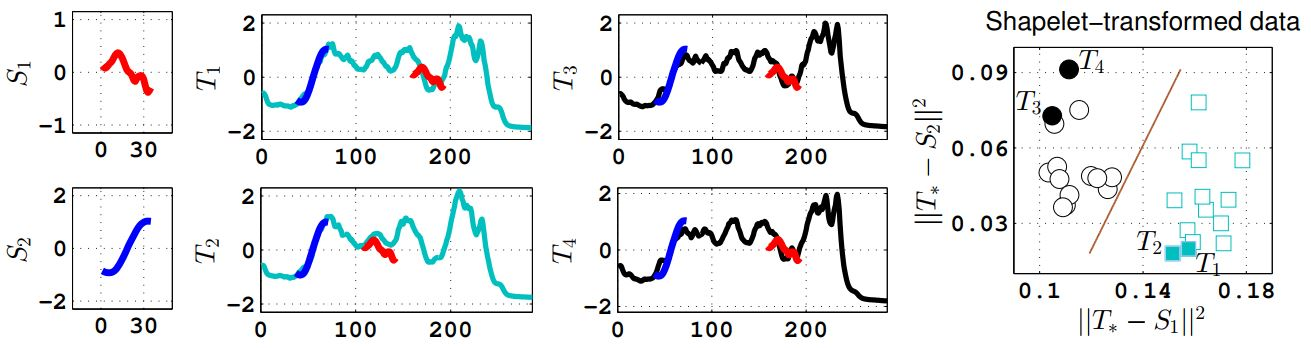
\includegraphics[scale = 0.45]{Shapelets.JPG}
    \centering
    \caption{An illustration of two shapelets S1, S2 (leftmost plots) learned on the Coffee dataset. Series’ distances to shapelets can optimally project the series into a 2-dimensional space, called the shapelet-transformed representation \cite{lines2012shapelet} (rightmost plot). The middle plots show the closest matches of the shapelets on series of two classes having light-blue and black colors \cite{grabocka2014learning}.}
    \label{Img:Shapelet}
\end{figure}

The original shapelet algorithm enumerated all possible shapelets and embeded the best ones, based on information gain assessment, in a decision tree.
Together with a calculated distance threshold, the shapelets and the threshold are used together as splitting criteria \cite{lines2018time,schafer2015boss}.
There have been many attempts to speed up the process of shapelets discovery, by determining good shapelets in a faster manner.
Two of them are; Fast Shapelets (FS) \cite{rakthanmanon2013fast} and Learned Shapelets (LS) \cite{grabocka2014learning}.
FS applied discretization through Symbolic Aggregate Approximation (SAX) to reduce the length of time series,
while LS tried to learn the shapelets \cite{shifaz2020ts}.
Later on the idea of tranforming time series data to an alternative space was adopted in \cite{hills2014classification},
the transformed data consists of distances to the best k shapelets, then classification is done using an ensemble of eight classifiers.

\subsubsection{Learned Shapelets}
\label{SubsubsectionLS}
Learned Shapelets (LS) was proposed in \cite{grabocka2014learning} as a new prospective for approaching time series shapelets.
Instead of searching for shapelets through enumeration of all candidates, LS learns K near-to-optimal shapelets that can linearly
separate instances through a stochastic gradient objective \cite{lines2018time,bostrom2018shapelet}.
The found shapelets need not to be a subsequence of one of the training examples \cite{bagnall2017great,schafer2017fast}.

LS follows a two steps technique. In the begining LS looks for a set of shapelets from the training data set using two parameters;
L controls the length of shapelets searched, while R controls the scaling of subsequences. Then these shapelets are clustered using
a K-Means algorithm and instances are represented in a new K-dimensional format where the values of the features represent the minimum
distance between the instance and one of the shapelets.

For the second step, using the new features representation, LS can start learning class probabilities for instances by considering a logistic regression model for each
of the classes and optimizing a regularized logistic loss function. The regularized loss function updates the shapelets and the weights of features.
This process keeps iteratively going untill either the model converges or the maximum number of iterations is reached.\cite{bostrom2018shapelet}.
In summary, the main objective of the aglorithm is to learn collectively the optimal shapelets and the weights
linear hyper-plane that minimizes the objective function \cite{bagnall2017great,grabocka2014learning}.

\subsubsection{Shapelet Transform}
\label{SubsubsectionST}
The first Shapelet Transform (ST) was introduced in \cite{hills2014classification}.
While the original algorithm embeded shapelets discovery in decision trees and assesed candidates through enumeration and 
the use Information Gain (IG) at each node, ST proposed a different way that saved repeating the brute force multiple times \cite{bostrom2018shapelet}.
ST seggregated the shapelets discovery process from the classifier. This seggregation opened the door for choosing classifiers freely and considering more accurate
classifiers than decision trees \cite{bagnall2017great,lines2015time}. Also \cite{hills2014classification} experimented with other shapelet assessment metrics like Kruskal-Wallis, F-stat and Mood’s median
to find out that F-stat attained higher accuracies than the other three and than IG \cite{bostrom2018shapelet}.

ST follows a three step procedure. In the beginning, a data transformation phase is carried out by utilizing a single-scan algorithm and extracting K best shapelets from the training
data set where K represents a cutoff threshold for the maximum number of shapelets to extract without affecting the quality of the shapelets extracted.
Then a reduction process is done by clustering the shapelets together untill they reach a user defined number.
Finally, The clustered shapelets are then used to transform the original datasest, by representing instances in terms of their disatances to each one of the extracted shapelets.
They experimented with different classifiers other than decision trees, these are; C4.5 tree, 1-NN, naive Bayes, Bayesian network, Random Forest, Rotation Forest, and support vector machine,
for which decision trees proved to be the worst among all, while support vector machine proved to be the best \cite{hills2014classification}.

ST was then extended again by \cite{Bostrom2017}, the intuition behind it was that the previously used assessment technique couldn't hanlde multi-class problems \cite{Bostrom2017}.
Instead of assessing shapelets that discriminate between all classes, they accomodated a one-vs-all technique so that shapelets are assessed on their ability to separate one class to all other classes.
They also introduced a balancing technique to represent each of the classes with the same number of shapelets \cite{bagnall2017great}.
For the classification, a combination of tree based, kernel based and probabilistic classifiers were used in an ensemble on the transformed data set \cite{shifaz2020ts,lines2018time}.
Each of the classifiers was given a weight based on it's training accuracy and the final classification used weighted voting \cite{Bostrom2017}.
Although ST has proved to be a competent accurate classifier, it suffers from high training-time complexity \cite{shifaz2020ts}.

ST is one of multiple classifier in the bigger ensemble HIVE-COTE \cite{lines2018time}.
It also is among the slowest components of the ensemble; due to the exhaustive shapelet enumeration which reaches a complexity of $O(n^{2} \centerdot l^{4})$,
where $n$ is the size of the data set and $l$ is the length of the time series \cite{shifaz2020ts}.
During a modification that was introduced in \cite{bagnall2020tale} for HIVE-COTE, some enhancements were applied to ST.
Some of these enhancements were new, others were already suggested before.
The first enhancement was to add a time contract; so that it limits the exhaustive enumeration process to happen only during the contracted time.
The value of the time contract is configured using a new added parameter.
The second enhancement was to train a Rotation Forest classifier on the transformed data instead of the mixed ensemble.

In the beginning of the training process, ST explores the number of shapelets that exist in the data set during the contract time, then approximates the number of shapelet
samples it can acquire from each time series.
Based on the results, it modifies the time of the model using a reinforcement learning technique.
For the shapelets sampling process a random search is executed. If the time contract is long enough, then all shapelets are considered.
Then, an evaluation process starts, where all the acquired samples are compared and filtered; to exclude redundant shapelets.
The filtered samples are then evaluated using information gain (IG); to keep the best distinctive shapelets of the classes.
For multi-class problems, a one vs all evaluation is carried out as per the suggestion by \cite{Bostrom2017}.
After that the weak shapelets are excluded and the remaining shapelets are merged into a pool and the transformation process starts.
Finally, the rotation forest classifier is trained.
In our framework, we use a contractable version of ST instead of the original. The implemented version allows for specifying a contrat time
and uses a random forest classifier.